% !TeX program = pdflatex
\documentclass[tikz,border=8pt]{standalone}
\usepackage{pgfplots}
\pgfplotsset{compat=1.16}
\definecolor{FigureBlue}{HTML}{2563EB}
\definecolor{FigureOrange}{HTML}{EA580C}
\definecolor{FigureGreen}{HTML}{16A34A}
\definecolor{FigurePurple}{HTML}{7C3AED}
\begin{document}
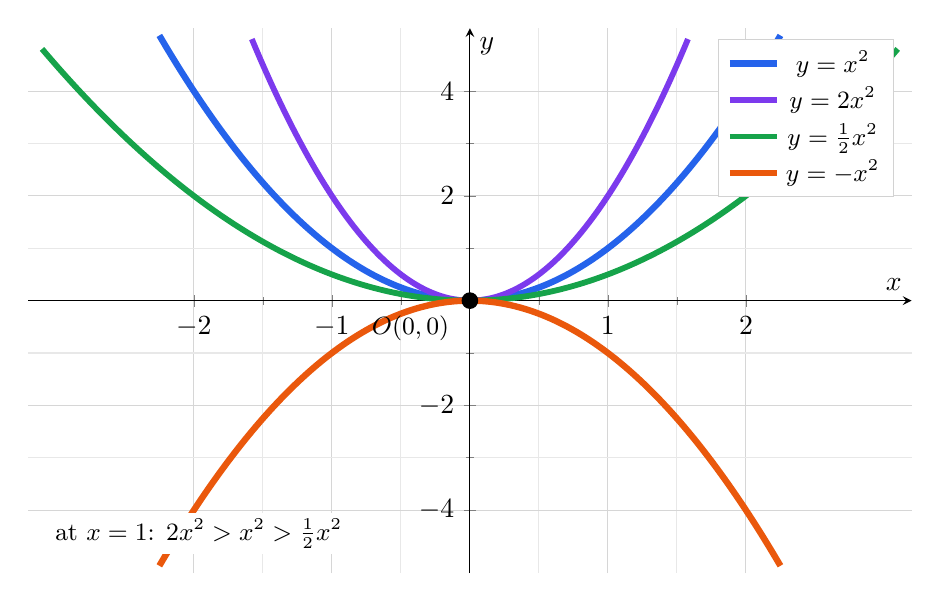
\begin{tikzpicture}
  \begin{axis}[
    width=12.8cm,height=8.5cm,
    axis lines=middle,
    xmin=-3.2,xmax=3.2,ymin=-5.2,ymax=5.2,
    xlabel={$x$},ylabel={$y$},
    xtick={-2,-1,0,1,2},ytick={-4,-2,0,2,4},
    grid=both,minor tick num=1,
    grid style={draw=gray!18},major grid style={draw=gray!32},
    legend style={at={(0.98,0.98)},anchor=north east,draw=gray!35,fill=white,font=\small},
    clip=false,
  ]
    \addplot[FigureBlue,line width=2.3pt,domain=-2.25:2.25,samples=181] {x^2};
    \addlegendentry{$y=x^2$}
    \addplot[FigurePurple,line width=2.1pt,domain=-1.58:1.58,samples=181] {2*x^2};
    \addlegendentry{$y=2x^2$}
    \addplot[FigureGreen,line width=2.1pt,domain=-3.1:3.1,samples=181] {.5*x^2};
    \addlegendentry{$y=\frac12x^2$}
    \addplot[FigureOrange,line width=2.3pt,domain=-2.25:2.25,samples=181] {-x^2};
    \addlegendentry{$y=-x^2$}
    \addplot[only marks,mark=*,mark size=2.8pt,black] coordinates {(0,0)};
    \node[anchor=north east,font=\small] at (axis cs:-.08,-.1) {$O(0,0)$};
    \node[anchor=south west,fill=white,inner sep=2pt,font=\small]
      at (axis cs:-3.05,-4.85) {at $x=1$: $2x^2>x^2>\frac12x^2$};
  \end{axis}
\end{tikzpicture}
\end{document}
